\section{\uppercase{Literature Review}}
In recent years, a lot of work has been done in mining hot/trending topics from Twitter stream. Twitter itself shows Trending Topics in its feed. \cite{lee2011twitter} have proposed extensions to this framework by classifying Trending Topics on Twitter using text-based and network-based classifiers. Recently, the focus in literature has shifted beyond the identification of trending topics; the problem of real-world event detection using social media has started receiving overwhelming attention. Researchers have explored the domain of event identification using social media updates, specifically Twitter. While some efforts have focused upon event detection in general \cite{becker2010learning}, other efforts have been directed towards detection of particular class of events such as earthquakes \cite{sakaki2010earthquake}, news reports \cite{sankaranarayanan2009twitterstand}. To this end, numerous techniques have been exploited. While \cite{becker2010learning} have explored ensemble-based clustering methods for learning similarity metrics for clustering related tweets, \cite{becker2011beyond} have focused on online identification of events using classification techniques. One special technique which has gained our attention, and which we have been exploring is using Topic Models on Twitter data for detection of events.

Topic modeling of the news-wire data has seen a lot of success. Topic modeling techniques such as LDA performs very well on the news data where a document is actually a mixture of a large number of topics. However, the standard LDA doesn't work well on the Twitter data, the major problem being that if we consider a tweet as a single document, then the document is too sparse for the LDA. The most commonly exploited technique to improve the performance of LDA on Twitter data is the aggregation of tweets which are similar in some sense or the other, such as temporally, linguistically, spatially and semantically, so as to feed the topic model with more content-rich documents enabling better topic inferences.

Several attempts have been made to extend LDA to better capture topics in micro-blogs and tweets. \cite{hong2010empirical} have analyzed different tweet aggregation techniques for training the topic models, in particular, LDA and the Author-Topic (AT) model \cite{rosen2004author}. The AT model extends LDA by modeling each word in the document as being latently associated to a topic $z$ as well as an author $x$. An author $x$ is a multinomial ($\theta$) over topics, which in turn is a multinomial distribution ($\phi$) over the words $w$ of the vocabulary. Unlike LDA, where only the words are observed, in AT model, both words and authors are observed. Three schemes have been discussed for training the topic models.
\begin{enumerate}
\item {\bf MSG scheme:} The focus here is the tweet itself. LDA is trained on all the tweets. For training purposes, each tweet is considered individually as a document.
\item {\bf USER scheme:} The focus here is the user. The model is not trained on individual tweets; rather, aggregation of all tweets of a particular user is fed to the model as a document.
\item {\bf TERM scheme:} This is a rather non-intuitive scheme, where tweets are aggregated based on the terms they contain. For each term, all the tweets containing that term are aggregated. Each document thus contains tweets that have a particular term in common.
\end{enumerate}

The inherent differences in the properties of each scheme can potentially lead to different topic proportions being inferred for the same testing set. For example, under \emph{MSG scheme}, model in trained on individual tweets, which are very short. Hence, more numbers of topics are needed for a reasonable performance. Training set for \emph{USER} and \emph{TERM schemes} have sufficiently large documents. The intuition behind the \emph{TERM scheme} is to capture the topics represented directly by the hashtags in tweets. Further, the authors use JS divergence to measure the similarity between the topics inferred by the three different schemes.

\cite{mehrotra2013improving} have examined additional tweet pooling schemes, including Burst-score wise pooling, Temporal pooling, and hashtag-based pooling. In Burst-score wise pooling, for each burst term, tweets possessing that term are pooled together into one document. Temporal pooling tries to capture the simultaneous tweets posted by users in wake of an occurrence of a major event by concatenating tweets posted within the same hour to form a document. The resulting topic inferences were found to be best in case of hashtag-based pooling. This result is quite intuitive, since hashtags inherently represent the context of the tweets; they are topics in disguise, and can be viewed as indirect topic assignment by the humans themselves. However, as noted, only a small portions of tweets are hash-tagged. Moreover, hash tags may not cover all the topics related to the tweet.

LDA as a model is unsupervised in nature. It does not need any labeled documents for the purpose of topic inferences. \cite{ramage2009labeled} have proposed Labeled LDA, a supervised version of the standard LDA, wherein a set of labels are provided as parameter to the model to be used as observed parameters for assigning topics to the documents. \cite{ramage2010characterizing} have explored the nature of Twitter messages and classified them into five different categories. Among these categories, the category of interest to us is the \emph{substance category}, which encompasses tweets about events, ideas, things, or people. They have used Labeled LDA to explore latent dimensions in Twitter posts, and further project these dimensions to the five categories. Further, to exploit the supervised learning aspect of Labeled LDA, they have used labels derived from hashtags, emoticons and Twitter meta-data like replies and temporal information to train the model. The combination of the latent features, and labeled features, and their projection to the \emph{substance category} could potentially lead to very accurate topic-to-event mapping which we are aiming to achieve.

 \begin{figure*}
 \centering
 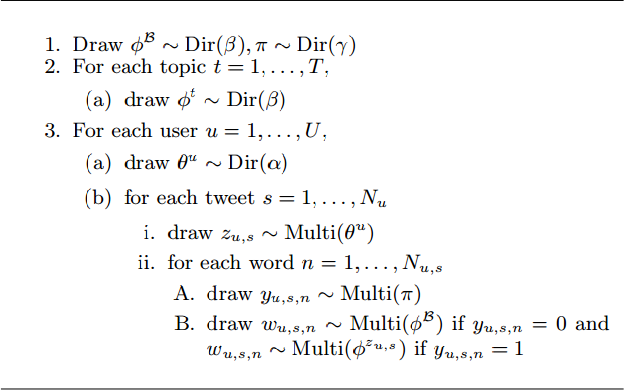
\includegraphics[width=0.6\textwidth]{figures/lda-algo}
 \caption{Twitter LDA Generative Process}
 \label{fig:twitterlda-algo}
\end{figure*}

Numerous research efforts have proposed approaches which are branches of the topic modeling paradigm, enhanced by use of other novel techniques and orthogonal ideas. \cite{wang2013real} have employed Gaussian mixture for choosing bursty words as potential candidates for being associated to an event. To further evaluate their candidacy, they have employed evolutionary clustering to model the temporal evolution of the candidate topics, before declaring them as being tightly-coupled to an event. They have proposed a time dependent HDP, which is an extension of a yet another powerful topic model - Hierarchical Dirichlet Process (HDP). Similarly, \cite{you2013geam} have come up with an Aspect Model called GEAM (General and Event-related Aspect Model) for extracting events information from noisy Twitter data.

With so many model proposals in the literature for event detection based on Twitter data, our focus is to tune the proposed models to fit our requirements - detection of non-popular events. While many methods are agnostic to popularity or bursty nature of the events being detected, others directly or indirectly focus on trending events. Our aim is to come up with suitable modifications to these approaches to remove their inherent inclination towards popular events and topics.

